% Options for packages loaded elsewhere
\PassOptionsToPackage{unicode}{hyperref}
\PassOptionsToPackage{hyphens}{url}
%
\documentclass[
]{article}
\usepackage{lmodern}
\usepackage{amssymb,amsmath}
\usepackage{ifxetex,ifluatex}
\ifnum 0\ifxetex 1\fi\ifluatex 1\fi=0 % if pdftex
  \usepackage[T1]{fontenc}
  \usepackage[utf8]{inputenc}
  \usepackage{textcomp} % provide euro and other symbols
\else % if luatex or xetex
  \usepackage{unicode-math}
  \defaultfontfeatures{Scale=MatchLowercase}
  \defaultfontfeatures[\rmfamily]{Ligatures=TeX,Scale=1}
\fi
% Use upquote if available, for straight quotes in verbatim environments
\IfFileExists{upquote.sty}{\usepackage{upquote}}{}
\IfFileExists{microtype.sty}{% use microtype if available
  \usepackage[]{microtype}
  \UseMicrotypeSet[protrusion]{basicmath} % disable protrusion for tt fonts
}{}
\makeatletter
\@ifundefined{KOMAClassName}{% if non-KOMA class
  \IfFileExists{parskip.sty}{%
    \usepackage{parskip}
  }{% else
    \setlength{\parindent}{0pt}
    \setlength{\parskip}{6pt plus 2pt minus 1pt}}
}{% if KOMA class
  \KOMAoptions{parskip=half}}
\makeatother
\usepackage{xcolor}
\IfFileExists{xurl.sty}{\usepackage{xurl}}{} % add URL line breaks if available
\IfFileExists{bookmark.sty}{\usepackage{bookmark}}{\usepackage{hyperref}}
\hypersetup{
  pdftitle={Statistical Inference Course Project Part2},
  pdfauthor={Kaaltho},
  hidelinks,
  pdfcreator={LaTeX via pandoc}}
\urlstyle{same} % disable monospaced font for URLs
\usepackage[margin=1in]{geometry}
\usepackage{color}
\usepackage{fancyvrb}
\newcommand{\VerbBar}{|}
\newcommand{\VERB}{\Verb[commandchars=\\\{\}]}
\DefineVerbatimEnvironment{Highlighting}{Verbatim}{commandchars=\\\{\}}
% Add ',fontsize=\small' for more characters per line
\usepackage{framed}
\definecolor{shadecolor}{RGB}{248,248,248}
\newenvironment{Shaded}{\begin{snugshade}}{\end{snugshade}}
\newcommand{\AlertTok}[1]{\textcolor[rgb]{0.94,0.16,0.16}{#1}}
\newcommand{\AnnotationTok}[1]{\textcolor[rgb]{0.56,0.35,0.01}{\textbf{\textit{#1}}}}
\newcommand{\AttributeTok}[1]{\textcolor[rgb]{0.77,0.63,0.00}{#1}}
\newcommand{\BaseNTok}[1]{\textcolor[rgb]{0.00,0.00,0.81}{#1}}
\newcommand{\BuiltInTok}[1]{#1}
\newcommand{\CharTok}[1]{\textcolor[rgb]{0.31,0.60,0.02}{#1}}
\newcommand{\CommentTok}[1]{\textcolor[rgb]{0.56,0.35,0.01}{\textit{#1}}}
\newcommand{\CommentVarTok}[1]{\textcolor[rgb]{0.56,0.35,0.01}{\textbf{\textit{#1}}}}
\newcommand{\ConstantTok}[1]{\textcolor[rgb]{0.00,0.00,0.00}{#1}}
\newcommand{\ControlFlowTok}[1]{\textcolor[rgb]{0.13,0.29,0.53}{\textbf{#1}}}
\newcommand{\DataTypeTok}[1]{\textcolor[rgb]{0.13,0.29,0.53}{#1}}
\newcommand{\DecValTok}[1]{\textcolor[rgb]{0.00,0.00,0.81}{#1}}
\newcommand{\DocumentationTok}[1]{\textcolor[rgb]{0.56,0.35,0.01}{\textbf{\textit{#1}}}}
\newcommand{\ErrorTok}[1]{\textcolor[rgb]{0.64,0.00,0.00}{\textbf{#1}}}
\newcommand{\ExtensionTok}[1]{#1}
\newcommand{\FloatTok}[1]{\textcolor[rgb]{0.00,0.00,0.81}{#1}}
\newcommand{\FunctionTok}[1]{\textcolor[rgb]{0.00,0.00,0.00}{#1}}
\newcommand{\ImportTok}[1]{#1}
\newcommand{\InformationTok}[1]{\textcolor[rgb]{0.56,0.35,0.01}{\textbf{\textit{#1}}}}
\newcommand{\KeywordTok}[1]{\textcolor[rgb]{0.13,0.29,0.53}{\textbf{#1}}}
\newcommand{\NormalTok}[1]{#1}
\newcommand{\OperatorTok}[1]{\textcolor[rgb]{0.81,0.36,0.00}{\textbf{#1}}}
\newcommand{\OtherTok}[1]{\textcolor[rgb]{0.56,0.35,0.01}{#1}}
\newcommand{\PreprocessorTok}[1]{\textcolor[rgb]{0.56,0.35,0.01}{\textit{#1}}}
\newcommand{\RegionMarkerTok}[1]{#1}
\newcommand{\SpecialCharTok}[1]{\textcolor[rgb]{0.00,0.00,0.00}{#1}}
\newcommand{\SpecialStringTok}[1]{\textcolor[rgb]{0.31,0.60,0.02}{#1}}
\newcommand{\StringTok}[1]{\textcolor[rgb]{0.31,0.60,0.02}{#1}}
\newcommand{\VariableTok}[1]{\textcolor[rgb]{0.00,0.00,0.00}{#1}}
\newcommand{\VerbatimStringTok}[1]{\textcolor[rgb]{0.31,0.60,0.02}{#1}}
\newcommand{\WarningTok}[1]{\textcolor[rgb]{0.56,0.35,0.01}{\textbf{\textit{#1}}}}
\usepackage{graphicx,grffile}
\makeatletter
\def\maxwidth{\ifdim\Gin@nat@width>\linewidth\linewidth\else\Gin@nat@width\fi}
\def\maxheight{\ifdim\Gin@nat@height>\textheight\textheight\else\Gin@nat@height\fi}
\makeatother
% Scale images if necessary, so that they will not overflow the page
% margins by default, and it is still possible to overwrite the defaults
% using explicit options in \includegraphics[width, height, ...]{}
\setkeys{Gin}{width=\maxwidth,height=\maxheight,keepaspectratio}
% Set default figure placement to htbp
\makeatletter
\def\fps@figure{htbp}
\makeatother
\setlength{\emergencystretch}{3em} % prevent overfull lines
\providecommand{\tightlist}{%
  \setlength{\itemsep}{0pt}\setlength{\parskip}{0pt}}
\setcounter{secnumdepth}{-\maxdimen} % remove section numbering

\title{Statistical Inference Course Project Part2}
\author{Kaaltho}
\date{20/12/2020}

\begin{document}
\maketitle

\hypertarget{synopsis}{%
\subsubsection{Synopsis}\label{synopsis}}

Now in the second portion of the project, we're going to analyze the
ToothGrowth data in the R datasets package.

Stages of the proyect.

1.Load the ToothGrowth data and perform some basic exploratory data
analyses Provide a basic summary of the data.

2.Use confidence intervals and/or hypothesis tests to compare tooth
growth by supp and dose. (Only use the techniques from class, even if
there's other approaches worth considering)

3.State your conclusions and the assumptions needed for your
conclusions.

\hypertarget{part-2-basic-inferential-data-analysis-instructions}{%
\subsubsection{\texorpdfstring{\textbf{Part 2: Basic Inferential Data
Analysis
Instructions}}{Part 2: Basic Inferential Data Analysis Instructions}}\label{part-2-basic-inferential-data-analysis-instructions}}

The first step is to simulate the variables that we want to compare.

\begin{Shaded}
\begin{Highlighting}[]
\CommentTok{#Oppening libraries}
\KeywordTok{library}\NormalTok{(ggplot2)}
\KeywordTok{library}\NormalTok{(cowplot)}

\CommentTok{#Assigning variables names, the specified data is the following:}
\KeywordTok{data}\NormalTok{(ToothGrowth)}
\KeywordTok{head}\NormalTok{(ToothGrowth)}
\end{Highlighting}
\end{Shaded}

\begin{verbatim}
##    len supp dose
## 1  4.2   VC  0.5
## 2 11.5   VC  0.5
## 3  7.3   VC  0.5
## 4  5.8   VC  0.5
## 5  6.4   VC  0.5
## 6 10.0   VC  0.5
\end{verbatim}

\textbf{\emph{Load the ToothGrowth data and perform some basic
exploratory data analyses Provide a basic summary of the data.}}

The next plot contains the distribution of the variables and it is
possible to see if it follows some distribution.

\begin{Shaded}
\begin{Highlighting}[]
\NormalTok{ToothGrowth}\OperatorTok{$}\NormalTok{dose<-}\KeywordTok{as.factor}\NormalTok{(ToothGrowth}\OperatorTok{$}\NormalTok{dose)}

\NormalTok{mean.supp =}\StringTok{ }\KeywordTok{split}\NormalTok{(ToothGrowth}\OperatorTok{$}\NormalTok{len, ToothGrowth}\OperatorTok{$}\NormalTok{supp)}
\KeywordTok{sapply}\NormalTok{(mean.supp, mean)}
\end{Highlighting}
\end{Shaded}

\begin{verbatim}
##       OJ       VC 
## 20.66333 16.96333
\end{verbatim}

\begin{Shaded}
\begin{Highlighting}[]
\NormalTok{mean.dose =}\StringTok{ }\KeywordTok{split}\NormalTok{(ToothGrowth}\OperatorTok{$}\NormalTok{len, ToothGrowth}\OperatorTok{$}\NormalTok{dose)}
\KeywordTok{sapply}\NormalTok{(mean.dose, mean)}
\end{Highlighting}
\end{Shaded}

\begin{verbatim}
##    0.5      1      2 
## 10.605 19.735 26.100
\end{verbatim}

\begin{Shaded}
\begin{Highlighting}[]
\CommentTok{#Ploting Type of Supplement versus the Tooth Length}
\CommentTok{#Changing as a factor}
\NormalTok{ToothGrowth}\OperatorTok{$}\NormalTok{dose<-}\KeywordTok{as.factor}\NormalTok{(ToothGrowth}\OperatorTok{$}\NormalTok{dose)}

\NormalTok{plot1 <-}\StringTok{ }\KeywordTok{ggplot}\NormalTok{(ToothGrowth, }\KeywordTok{aes}\NormalTok{(}\DataTypeTok{x=}\NormalTok{supp, }\DataTypeTok{y=}\NormalTok{len)) }\OperatorTok{+}
\StringTok{  }\KeywordTok{geom_boxplot}\NormalTok{(}\DataTypeTok{colour=}\StringTok{"darkviolet"}\NormalTok{, }\DataTypeTok{fill=}\StringTok{"skyblue"}\NormalTok{)}\OperatorTok{+}\StringTok{ }
\StringTok{  }\KeywordTok{guides}\NormalTok{(}\DataTypeTok{fill=}\OtherTok{FALSE}\NormalTok{) }\OperatorTok{+}
\StringTok{  }\KeywordTok{labs}\NormalTok{(}\DataTypeTok{x=}\StringTok{"Method of Supplement"}\NormalTok{, }\DataTypeTok{y=}\StringTok{"Tooth Length"}\NormalTok{, }\DataTypeTok{title=}\NormalTok{(}\StringTok{"Mean in legnth by Method supplement"}\NormalTok{))}\OperatorTok{+}
\StringTok{  }\KeywordTok{theme}\NormalTok{(}\DataTypeTok{plot.title =} \KeywordTok{element_text}\NormalTok{(}\DataTypeTok{hjust =} \FloatTok{0.5}\NormalTok{))}
  
  
\NormalTok{plot2 <-}\StringTok{ }\KeywordTok{ggplot}\NormalTok{(ToothGrowth, }\KeywordTok{aes}\NormalTok{(}\DataTypeTok{x=}\NormalTok{dose, }\DataTypeTok{y=}\NormalTok{len)) }\OperatorTok{+}
\StringTok{  }\KeywordTok{geom_boxplot}\NormalTok{(}\DataTypeTok{colour=}\StringTok{"darkviolet"}\NormalTok{, }\DataTypeTok{fill=}\StringTok{"skyblue"}\NormalTok{)}\OperatorTok{+}\StringTok{ }
\StringTok{  }\KeywordTok{guides}\NormalTok{(}\DataTypeTok{fill=}\OtherTok{FALSE}\NormalTok{) }\OperatorTok{+}
\StringTok{  }\KeywordTok{labs}\NormalTok{(}\DataTypeTok{x=}\StringTok{"Dose"}\NormalTok{, }\DataTypeTok{y=}\StringTok{"Tooth Length"}\NormalTok{, }\DataTypeTok{title=}\NormalTok{(}\StringTok{"Mean in length by dose"}\NormalTok{))}\OperatorTok{+}
\StringTok{  }\KeywordTok{theme}\NormalTok{(}\DataTypeTok{plot.title =} \KeywordTok{element_text}\NormalTok{(}\DataTypeTok{hjust =} \FloatTok{0.5}\NormalTok{))}

\CommentTok{#This plot is just one image with two plots on it}
\KeywordTok{plot_grid}\NormalTok{(plot1, plot2, }\DataTypeTok{align =} \StringTok{"v"}\NormalTok{, }\DataTypeTok{ncol =}\DecValTok{2}\NormalTok{, }\DataTypeTok{rel_heights =} \KeywordTok{c}\NormalTok{(}\DecValTok{1}\OperatorTok{/}\DecValTok{2}\NormalTok{, }\DecValTok{1}\OperatorTok{/}\DecValTok{2}\NormalTok{))}
\end{Highlighting}
\end{Shaded}

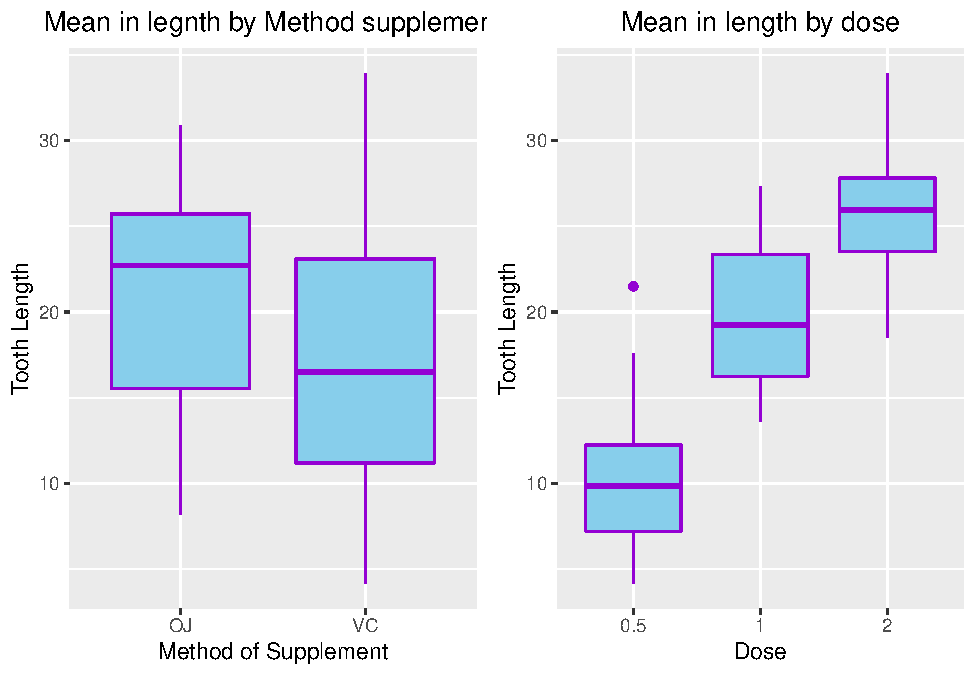
\includegraphics{Statistical-Inference-Course-Project-2_files/figure-latex/means-1.pdf}

As can be seen in the graph the distribution of the data of Method of
supplement OJ the mean is 20.63 while the mean of the Method of
supplement VC correspond to 16.93 length of teeth, apparently supplement
OJ has more Tooth Length measure than the Supplement VC. Considering the
distribution of Tooth Length relative to dose, it is possible to see
that a Dose of 2 have better Tooth length. Could be possible to infer
that an OJ method + 2 type dose could drive the results to a better
tooth development.

\textbf{\emph{Use confidence intervals and/or hypothesis tests to
compare tooth growth by supp and dose. (Only use the techniques from
class, even if there's other approaches worth considering)}}

Comparing tooth growth by supplement using a t-test.

\begin{Shaded}
\begin{Highlighting}[]
\KeywordTok{t.test}\NormalTok{(len}\OperatorTok{~}\NormalTok{supp,}\DataTypeTok{data=}\NormalTok{ToothGrowth)}
\end{Highlighting}
\end{Shaded}

\begin{verbatim}
## 
##  Welch Two Sample t-test
## 
## data:  len by supp
## t = 1.9153, df = 55.309, p-value = 0.06063
## alternative hypothesis: true difference in means is not equal to 0
## 95 percent confidence interval:
##  -0.1710156  7.5710156
## sample estimates:
## mean in group OJ mean in group VC 
##         20.66333         16.96333
\end{verbatim}

Due to the fact that the p-value is greater than 0.05 and the confidence
interval contains zero, it could be said that the supplement types does
not have a impact on Tooth growth.

Testing the tooth length by the group with vitamin C dosage

\begin{Shaded}
\begin{Highlighting}[]
\KeywordTok{t.test}\NormalTok{(ToothGrowth}\OperatorTok{$}\NormalTok{len[ToothGrowth}\OperatorTok{$}\NormalTok{dose}\OperatorTok{==}\DecValTok{2}\NormalTok{],ToothGrowth}\OperatorTok{$}\NormalTok{len[ToothGrowth}\OperatorTok{$}\NormalTok{dose}\OperatorTok{==}\DecValTok{1}\NormalTok{], }\DataTypeTok{paired =} \OtherTok{FALSE}\NormalTok{, }\DataTypeTok{var.equal =} \OtherTok{TRUE}\NormalTok{)}
\end{Highlighting}
\end{Shaded}

\begin{verbatim}
## 
##  Two Sample t-test
## 
## data:  ToothGrowth$len[ToothGrowth$dose == 2] and ToothGrowth$len[ToothGrowth$dose == 1]
## t = 4.9005, df = 38, p-value = 1.811e-05
## alternative hypothesis: true difference in means is not equal to 0
## 95 percent confidence interval:
##  3.735613 8.994387
## sample estimates:
## mean of x mean of y 
##    26.100    19.735
\end{verbatim}

\textbf{\emph{State your conclusions and the assumptions needed for your
conclusions.}}

Seeing that the p-value is approximately zero, can be said that there is
evidence to reject the null hypothesis. It is possible to say that
higher doses result in greater tooth growth.

Can be concluded that the Method of supplement doesn't have an
noticeable impact on tooth growth, furthermore dose level appear to have
an influence over tooth growth.

\end{document}
